\documentclass[a4paper,11pt]{report}
\usepackage[showexo=true,showcorr=false]{../packages/coursclasse}
%\usepackage{pstricks-add}

\toggletrue{montrerNiveaux}

\usepackage{enumitem}
\setlist[enumerate]{align=left,leftmargin=1cm,itemsep=10pt,parsep=0pt,topsep=0pt,rightmargin=0.5cm}
\setlist[itemize]{align=left,labelsep=1em,leftmargin=*,itemsep=0pt,parsep=0pt,topsep=0pt,rightmargin=0cm}

\setlength\columnsep{20pt}
\begin{document}

\newcommand{\chapterName}{Fonctions et algèbre}
\newcommand{\serieName}{Calcul littéral}

\chapter*{\chapterName}
\thispagestyle{empty}

\begin{amL}{\serieName}{
\item Expression littérale (page 67)
\item Alléger l'écriture d'expressions littérales (page 67)
\item Egalité de deux expressions littérales (page 68)
\item Monôme (page 68)
\item Degré d'un monôme (page 68)
}
\end{amL}
\section*{\serieName}
\setcounter{page}{1}
\thispagestyle{firstPage}


\vspace{-0.5cm}
%Connaissance et utilisation des règles et conventions usuelles d'écriture algébrique (Niv 2s-3s)
%Détermination de la valeur numérique d'une expression littérale (, 4x +5, abc, x3 …) en substituant des nombres aux lettres (Niv 2-3)
%Élaboration d'expressions littérales à partir de figures géométriques ou d'expressions verbales (Niv 2s-3s). • d’énoncés de problèmes, de figures géométriques ou d’expressions verbales.La répartition de cette progression suit celle des expressions étudiées

\begin{QSJ}{92}{2}
\end{QSJ}

\begin{resolu}{Coefficient}
{ 
\vspace{-0.2cm}
	Complète le tableau ci-dessous~:
\vspace{-0.2cm}
\begin{center}
%\resizebox{\columnwidth}{!}{
\begin{tabular}{|c|c|c|}
 \hline
   Monôme & Coefficient & Partie littérale\\   
\hline
$ 5x^2 $ &    $5$  & $x^2$ \\
 \hline
$a^3$ &$1$&$a^3$ \\
\hline  
\end{tabular}%}  
\end{center}
\vspace{-0.6cm}
}
{2}
\end{resolu}

\vspace{-0.2cm}
\begin{exop}
{
\vspace{-0.2cm}
	Complète le tableau ci-dessous~:
\vspace{-0.2cm}
\begin{center}
%\resizebox{\columnwidth}{!}{
\begin{tabular}{|c|c|c|}
 \hline
   Monôme & Coefficient & Partie littérale\\   
\hline
$25x$ &    &  \\
 \hline
$3a^2$ &  & \\
\hline 
 & $1$ & $b$ \\
\hline
$1$&&\\
\hline
$-8x^3$&&\\
\hline  
   \rule{0pt}{4ex}\rule[-2ex]{0pt}{0ex}
$\dfrac{1}{5}c^3$ &  & \\
\hline  
\end{tabular}%  }
\end{center}
\vspace{-0.6cm}
}
{2}
\end{exop}

\vspace{-0.2cm}
\begin{exop}
{
\vspace{-0.2cm}
	Complète le tableau ci-dessous~:
\vspace{-0.2cm}
\begin{center}
%\resizebox{\columnwidth}{!}{
\begin{tabular}{|c|c|c|}
 \hline
   Monôme & Coefficient & Partie littérale\\   
\hline
$x$ &    &  \\
\hline 
   \rule{0pt}{4ex}\rule[-2ex]{0pt}{0ex}
 & $\dfrac{3}{4}$ & $a^3$ \\
\hline 
   $-x^2$ &  & \\
\hline 
 & $0$ &  \\
\hline  
$b^3$ &  & $b^3$ \\
\hline  
\end{tabular} % }
\end{center}
\vspace{-0.6cm}
}
{2}
\end{exop}

%convention

\begin{resolu}{Conventions}
{ Relie chaque expression à sa forme réduite~:
\begin{center}
	\begin{tabular}{rc@{\hspace{4cm}}c@{}cl}
$x \cdot x \cdot x$ & $\bullet$ &\hspace{5cm}& $\bullet$ & $7x+3y$\\
$3 \cdot x + 1$ & $\bullet$ &\hspace{5cm}& $\bullet$ & $3x+1$\\
$7 \cdot x + 3\cdot y$ & $\bullet$ &\hspace{5cm}& $\bullet$ &$x^3$
\end{tabular}
\end{center}
}
{2}
\end{resolu}


\begin{exop}
{Relie chaque expression à sa forme réduite~:~:
\begin{center}
\begin{tabular}{rc@{\hspace{4cm}}c@{}cl}
$x \cdot x$ & $\bullet$ &\hspace{5cm}& $\bullet$ & $y^3$\\
$x \cdot y + 3\cdot y$ & $\bullet$ &\hspace{5cm}& $\bullet$ & $\dfrac{5}{3}x$\\
$y \cdot y \cdot y$ & $\bullet$ &\hspace{5cm}& $\bullet$ &$x^2$\\
$1 \cdot x$ & $\bullet$ &\hspace{5cm}& $\bullet$ & $x$\\
$0 \cdot y + 4$ & $\bullet$ &\hspace{5cm}& $\bullet$ &$xy+3y$\\
$\dfrac{5}{3} \cdot x$ & $\bullet$ &\hspace{5cm}& $\bullet$ &$4$
\end{tabular}
\end{center}
}
{2}
\end{exop}

\begin{exop}
{Relie chaque expression à sa forme réduite~:
	\begin{center}
\begin{tabular}{rc@{\hspace{4cm}}c@{}cl}
		$3 \cdot x - 7 \cdot x $ & $\bullet$ &\hspace{5cm}& $\bullet$ & $ y^3+xy$\\
		$x \cdot y + 3x\cdot y$  & $\bullet$ &\hspace{5cm}& $\bullet$ & $x+4y$\\
 $y \cdot y \cdot y + y\cdot x$ & $\bullet$ &\hspace{5cm}& $\bullet$ &$-4x$\\
 $1 \cdot x + 4\cdot y$ & $\bullet$ &\hspace{5cm}& $\bullet$ &$x^3+x$\\
 $ x \cdot x \cdot x + x$ & $\bullet$ &\hspace{5cm}& $\bullet$ &$4xy$
\end{tabular}
\end{center}
}
{3}
\end{exop}

\begin{exop}{Simplifie, si possible, les expressions suivantes~:
\begin{tasks}
    \task $3\cdot x$ ~:\hrulefill
    \task $3\cdot 4$ ~:\hrulefill
     \task $1\cdot x$ ~:\hrulefill
     \task $1+ x$ ~:\hrulefill
    \task  $0\cdot x$ ~:\hrulefill
    \task  $3\cdot x + 4\cdot y$ ~:\hrulefill 
    \task  $x\cdot x$ ~:\hrulefill    
\end{tasks}
}
{3}
\end{exop}

\begin{exop}{Simplifie, si possible, les expressions suivantes~:
\begin{tasks}
    \task $5\cdot g$ ~:\hrulefill
    \task $g\cdot g$ ~:\hrulefill
    \task $1\cdot g$ ~:\hrulefill
    \task $0\cdot g$ ~:\hrulefill
    \task $3\cdot 6$ ~:\hrulefill
    \task $1\cdot g + 4$ ~:\hrulefill
    \task $2\cdot g + 3\cdot h$ ~:\hrulefill
\end{tasks}
}
{4}
\end{exop}

%relie chaque expression à sa forme réduite.
\begin{exof}{fa73}{97}{2}
\end{exof}
\begin{exof}{fa74}{97}{2}
\end{exof}
\begin{exof}{fa75}{98}{2}
\end{exof}

\begin{resolu}{Vocabulaire}{Écris l'expression algébrique correspondant à chaque phrase~:
		\vspace{-0.3cm}
\begin{tasks}[after-item-skip = 0.2em]
    \task un nombre augmenté de 5~: $x+5$
    \task le double d'un nombre~: $2x$
    \task le carré d'un nombre~: $x^2$
\end{tasks}
\vspace{-0.3cm}
}
{2}
\end{resolu}

\begin{exop}{Écris l'expression algébrique correspondant à chaque phrase~:
		\vspace{-0.3cm}
\begin{tasks}[after-item-skip = 0.3em]
    \task la somme de $x$ et 4~: \hrulefill
     \task  la différence de 6 et $x$~: \hrulefill
     \task  le cube de $x$~: \hrulefill
    \task  le quotient de $x$ par 5~: \hrulefill
\end{tasks}
\vspace{-0.3cm}
}
{2}
\end{exop}

\begin{exof}{FA65}{94}{2}
\end{exof}

\begin{exol}{FA63}{89}{2}
\end{exol}

\begin{exop}{ Écris l'expression algébrique correspondant à chaque phrase~:
		\vspace{-0.3cm}
\begin{tasks}[after-item-skip = 0.3em]
    \task La différence du cube de $x$ et de 3~: \hrulefill
    \task La somme du quotient de $x$ par 4 et du carré de $y$~: \hrulefill
     \task  Le quotient de $x$ par le cube de $y$~: \hrulefill
     \task  La somme du produit de $x$ par $y$ et du triple de $x$~: \hrulefill
    \task  Le produit de 5 par la somme de $x$ et $z$~: \hrulefill
\end{tasks}
\vspace{-0.3cm}
}
{3}
\end{exop}

\begin{exop}{ Traduis chaque expression littérale par une phrase~:
\begin{tasks}
    \task $x^3-4$~: \hrulefill
    \task $(x+3)\cdot5$~: \hrulefill
     \task  $\dfrac{1}{3}x$~: \hrulefill
     \task  $(x^2+3)\cdot2$~: \hrulefill
\end{tasks}
}
{3}
\end{exop}
%lier une expression à son voc

\begin{exof}{FA66}{94}{2}
\end{exof}

\begin{exol}{FA67}{89}{2}
\end{exol}

\begin{exol}{FA82}{91}{2}
\end{exol}

\begin{exol}{FA83}{91}{2}
\end{exol}

%substitution
\begin{resolu}{Substitution}
{Calcule la valeur de l'expression si $x=2$.
	\vspace{-0.3cm}
\begin{tasks}(2)
    \task $2x+4 = 2\cdot 2 + 4= 8$
    \task $x(x^2 + 3)= 2\cdot (2^2 + 3)=2 \cdot 7 =14$
\end{tasks}
}
{2}
\end{resolu}

\begin{exo}
{Calcule la valeur de l'expression si $x=3$.
	\vspace{-0.3cm}
\begin{tasks}(4)
    \task $10x-3=$
     \task $5x^2=$
     \task $7x+3=$
     \task $5+\dfrac{5x}{2}=$
\end{tasks}
}
{2}
\end{exo}

\begin{exo}
{Calcule la valeur de l'expression si $x=2$ et $y=5$.
\begin{tasks}(4)
    \task $10x-y=$
     \task $3x^2-2y=$
     \task $x-3y=$
     \task $y+\dfrac{5x}{2}=$
\end{tasks}
\vspace{-0.3cm}
}
{2}
\end{exo}


\begin{exo}
{Calcule la valeur de l'expression si $x=5$ et $y=3$.
\begin{tasks}(2)
    \task $2x+3y=$
     \task $xy+5=$
     \task $x^2+(5-y)=$
     \task $3x+2xy-7=$
\end{tasks}
}
{2}
\end{exo}

\begin{exo}
{Calcule la valeur de l'expression si $x=7$ et $y=3$.
\begin{tasks}(2)
    \task $2x-(3y-4)=$
     \task $3(xy-5)=$
     \task $100-(2xy+9)=$
     \task $(3x^2-5)\cdot2=$
\end{tasks}
}
{2}
\end{exo}

\begin{exo}
{Calcule la valeur de l'expression si $x=3$ et $y=2$.
\begin{tasks}(2)
    \task $(2x+y)(x-y)=$
     \task $50-(xy+4)(x+y)=$
     \task $2(x+y)\cdot5=$
     \task $x(3+x)^2=$
\end{tasks}
}
{2}
\end{exo}


\begin{exo}
{Voici une série d'égalités. Pour chacune d'entre elles, détermine si elle est toujours vraie (TV) quelle que soit la valeur donnée à $x$, parfois vraie (PV), ou si aucune valeur de $x$ ne permettra d'obtenir une égalité, c'est à dire toujours fausse (TF).
\begin{tasks}(2)
    \task $2x+2=8$
     \task $5x=x+4$
     \task $9x=6x+3x$
     \task $15x-5=25$
     \task $x-5=x+5$
     \task $3+2x=5x-3x+3$
\end{tasks}
}
{2}
\end{exo}

\begin{exof}{FA70}{96}{2}
\end{exof}

\begin{exof}{FA71}{96}{2}
\end{exof}

\begin{exol}{FA69}{89}{2}
\end{exol}

%donner l'équation

\begin{resolu}{Expression algébrique}
{

	\begin{minipage}[t]{0.5\textwidth}{
	\vspace{0pt}
	Donne l'expression algébrique du périmètre et de l'aire du rectangle suivant~:
	}
	\end{minipage}
	\hfill
	\begin{minipage}[t]{0.4\textwidth}{
	\vspace{0pt}
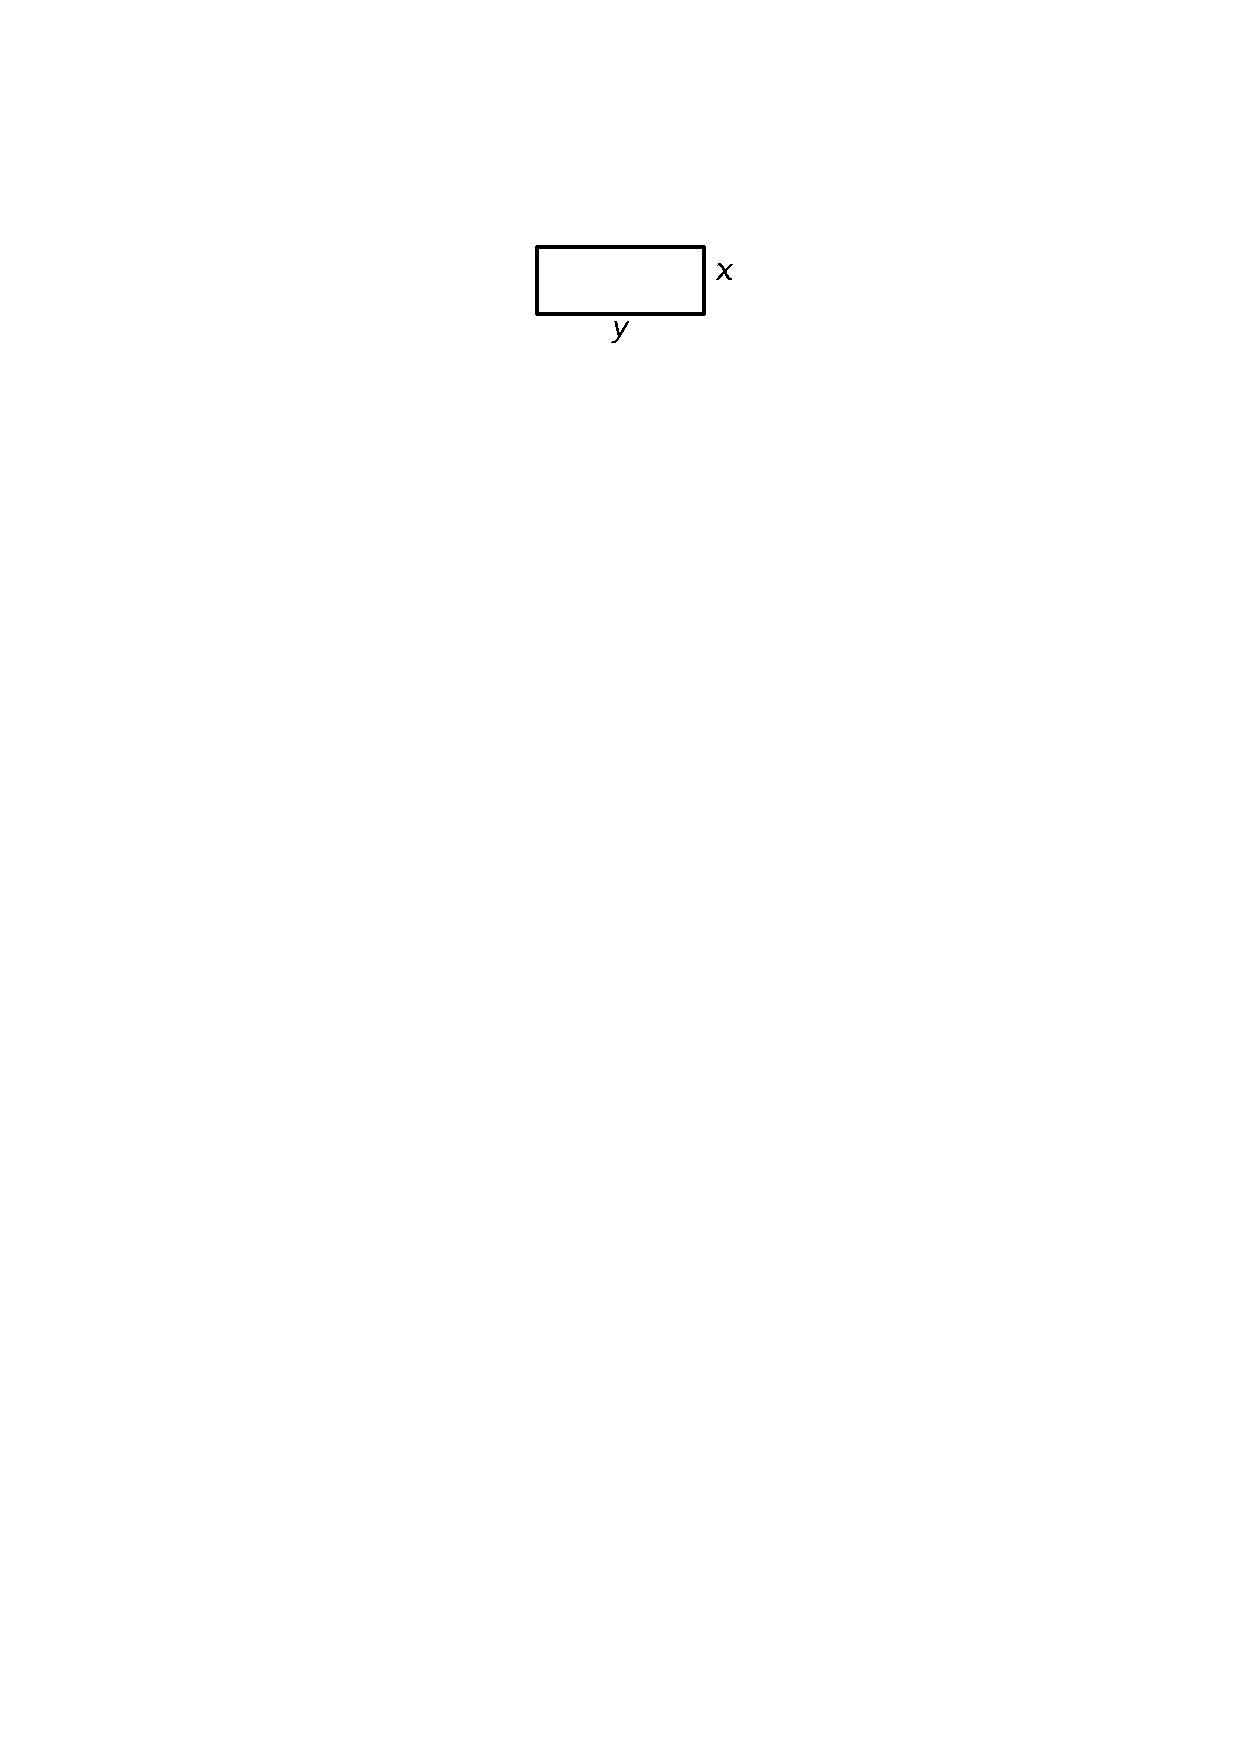
\includegraphics[scale=1.2]{media/fa-10/rectangle.pdf}
	}
	\end{minipage}\begin{center}	
\end{center}

L'expression algébrique du périmètre du rectangle est~:

$x+x+y+y$

et celle de l'aire est~:

$x \cdot y =xy$
}
{2}
\end{resolu}

\begin{exop}{ Donne l'expression algébrique des périmètres et aires de ces figures en fonction de $x, y, z$ et $h$~:

\begin{tasks}(2)
	\task[] 
Périmètre = \hrulefill

    Aire = \hrulefill

\begin{center}
	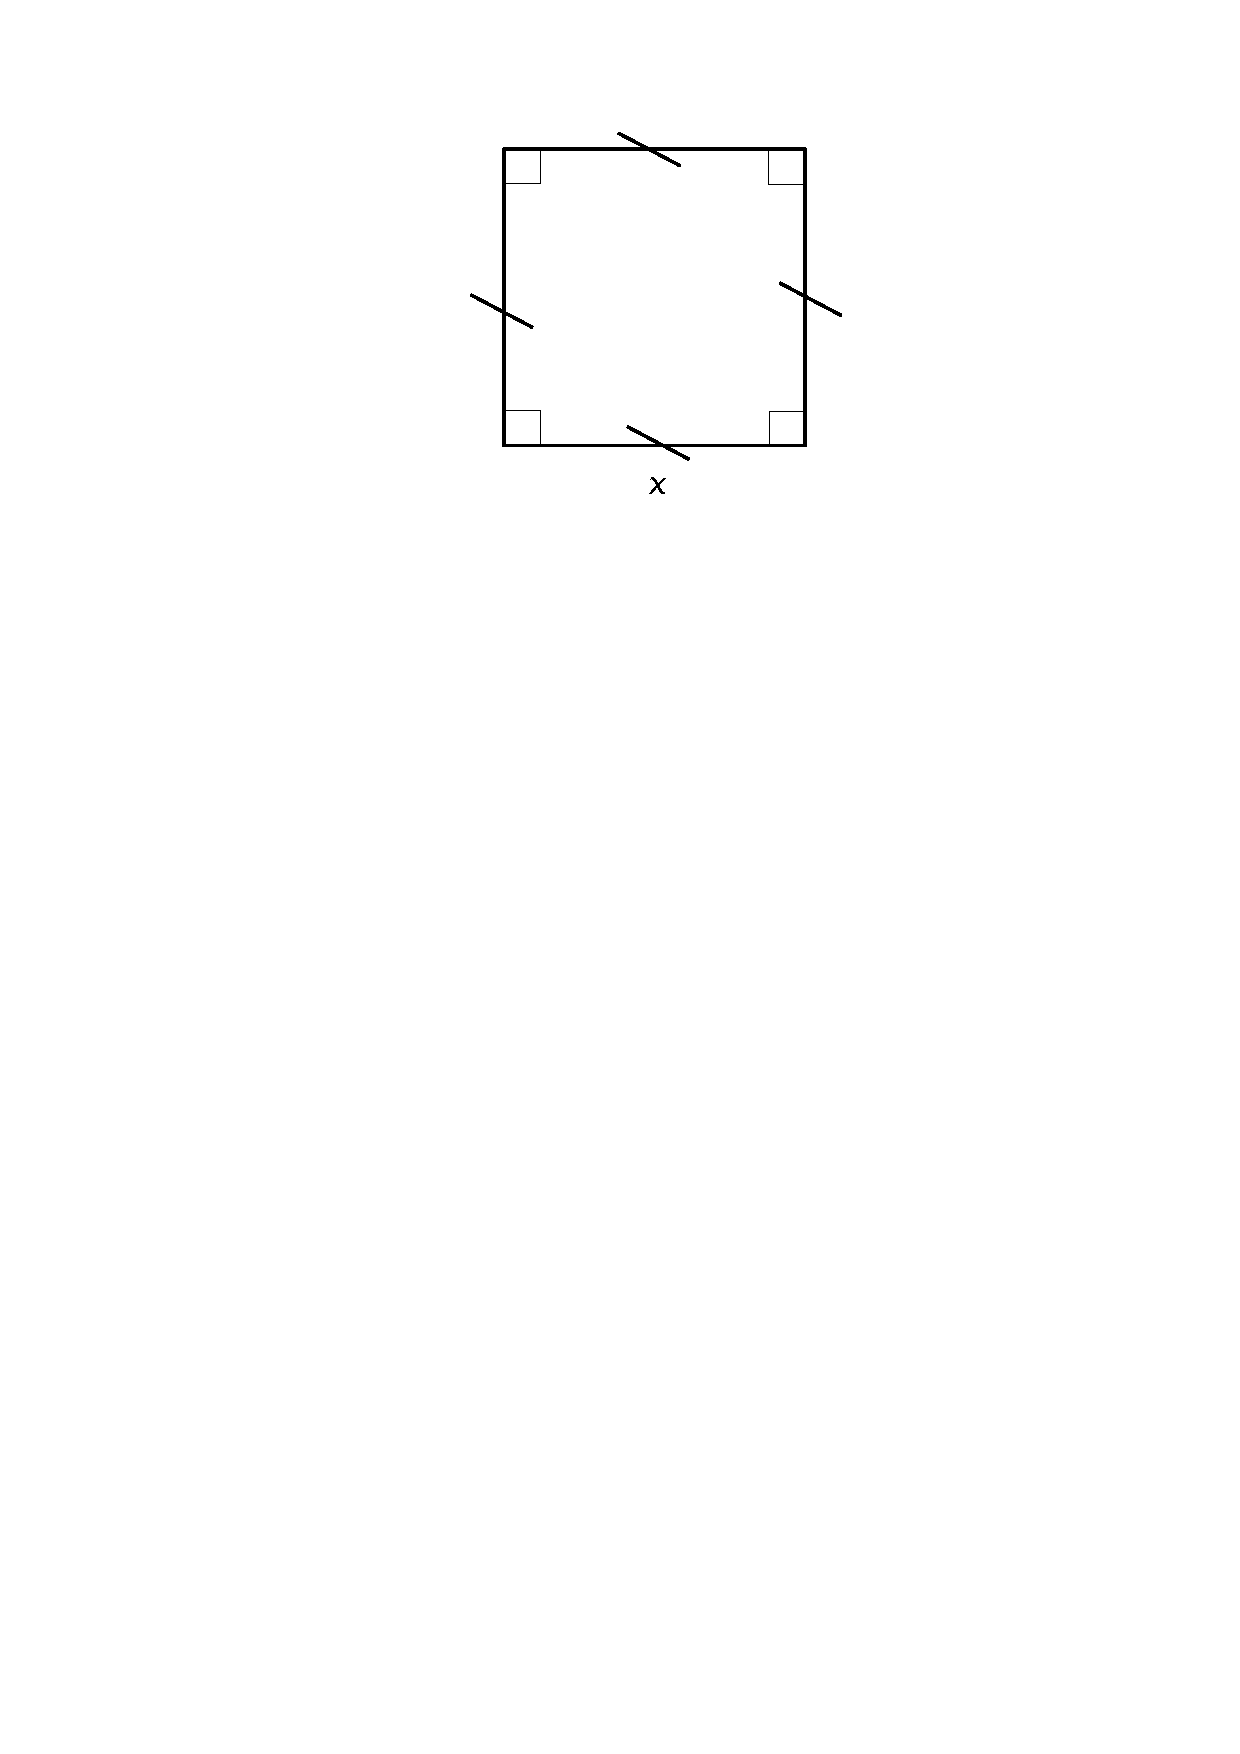
\includegraphics[scale=0.7]{media/fa-10/carre.pdf}
\end{center}

    \task[]
Périmètre = \hrulefill

 Aire = \hrulefill
 
     \begin{center}
     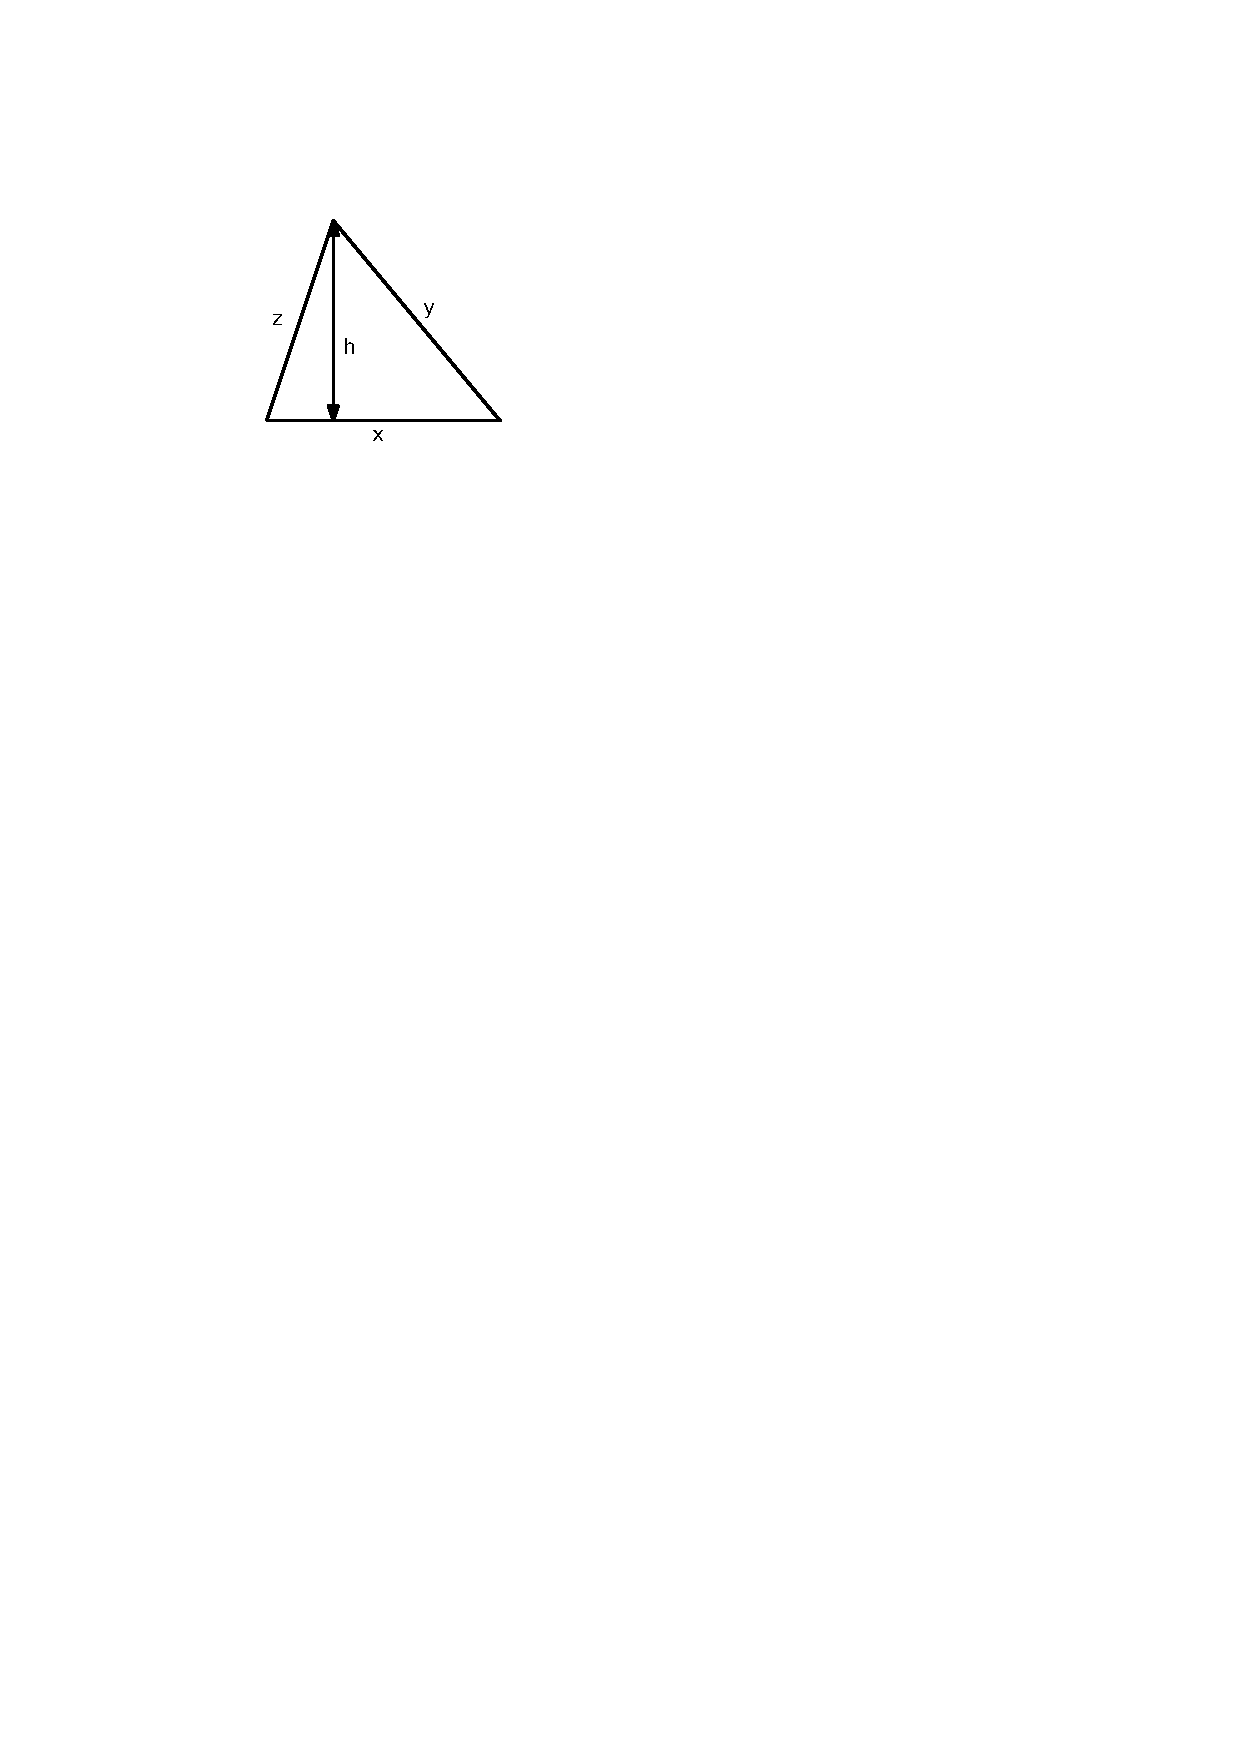
\includegraphics[scale=1.0]{media/fa-10/triangle.pdf}
\end{center}

\end{tasks}

  
}
{3}
\end{exop}

\begin{exop}{ 
\begin{minipage}[t]{0.5\textwidth}{
\vspace{0pt}
Donne l'expression algébrique du périmètre de cette figure en fonction de $x$, $y$ et $z$~:
}
\end{minipage}
\begin{minipage}[t]{0.5\textwidth}{
\vspace{0pt}
\begin{center}    
     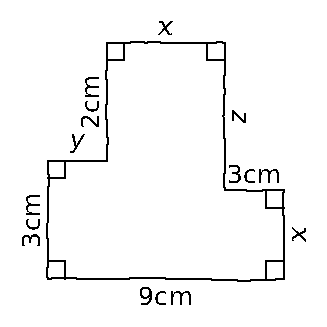
\includegraphics[scale=0.9]{media/fa-10/calclit}
\end{center}
}
\end{minipage}




Périmètre = \hrulefill
  
}
{3}
\end{exop}

\begin{exop}{ Donne l'expression algébrique de la longueur du segment $AB$ en fonction de $x$~:

\begin{tasks}(2)
    \task 
    
    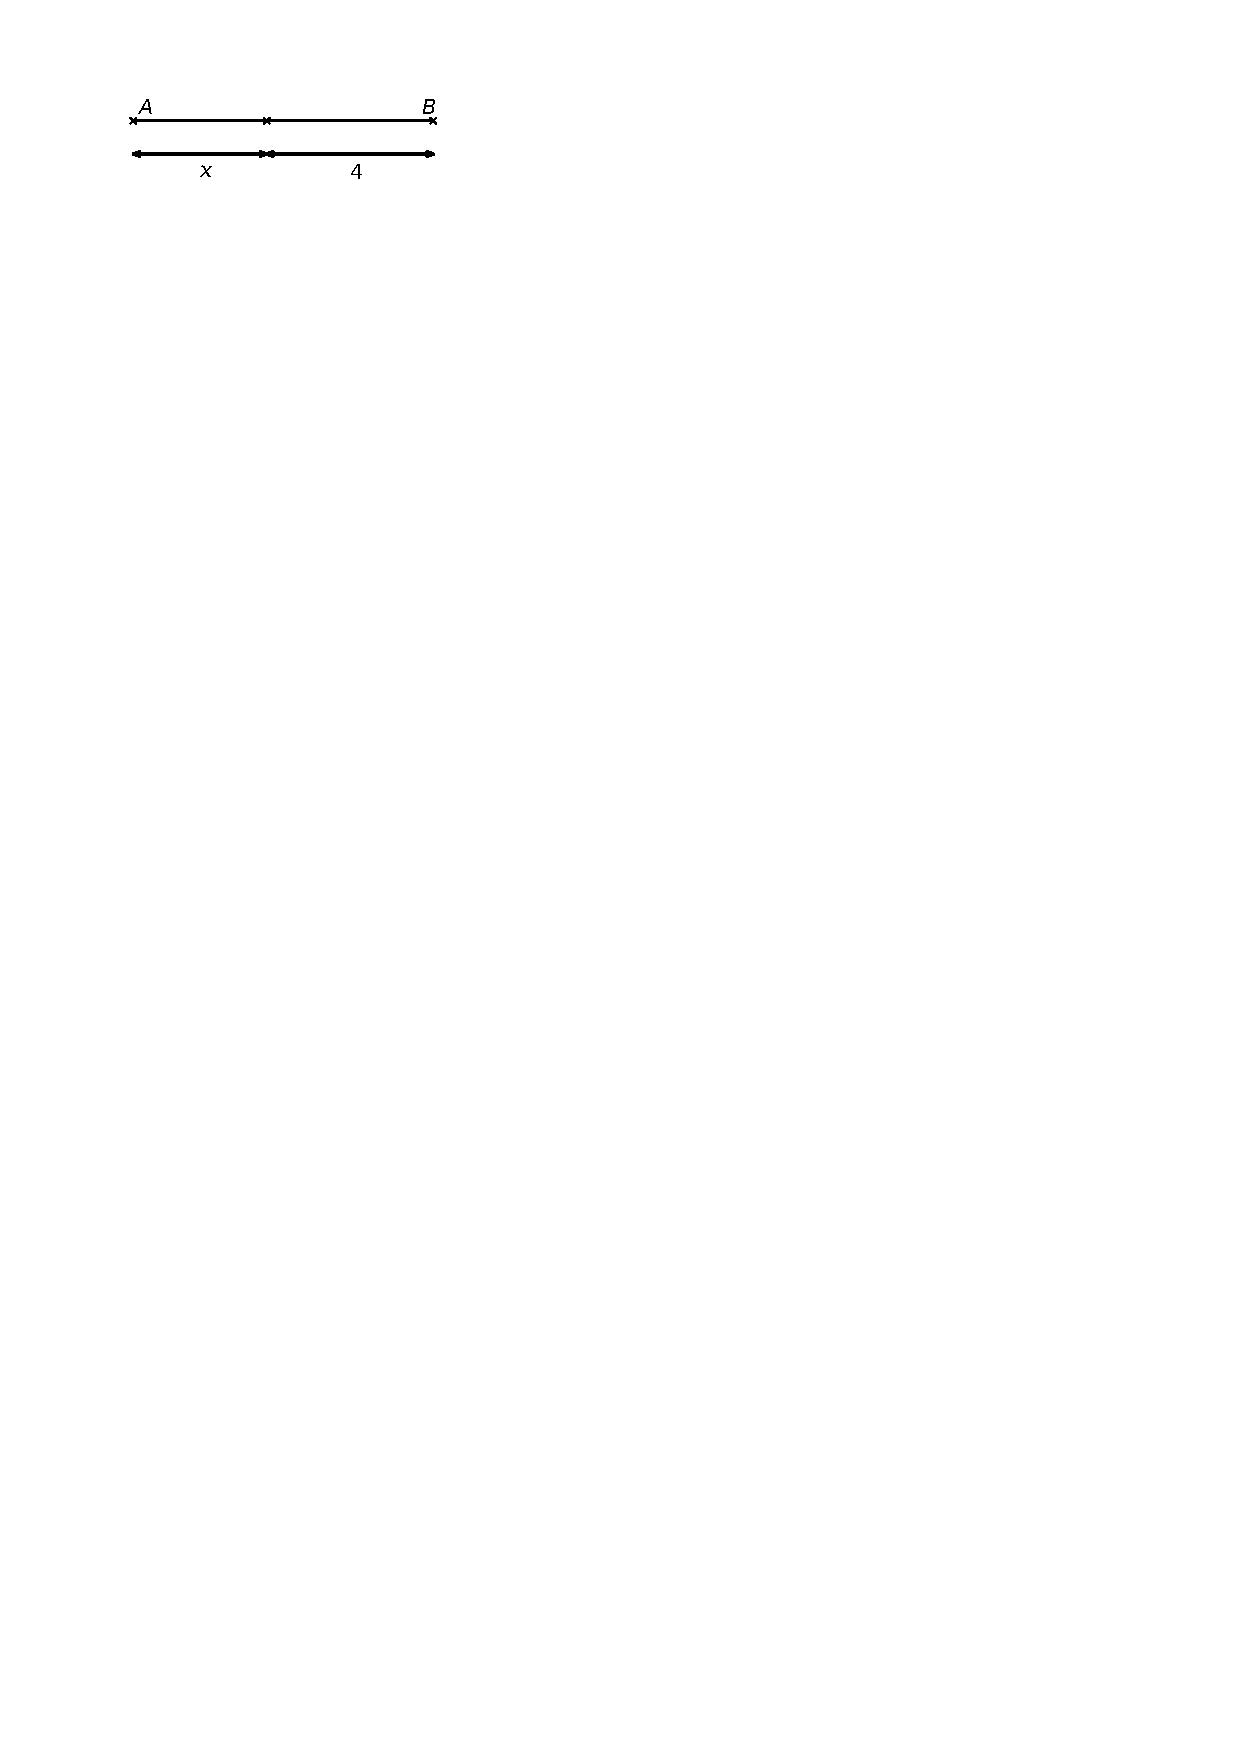
\includegraphics[scale=1.2
    ]{media/fa-10/ligne1.pdf}

AB = \hrulefill
  \task 
  
     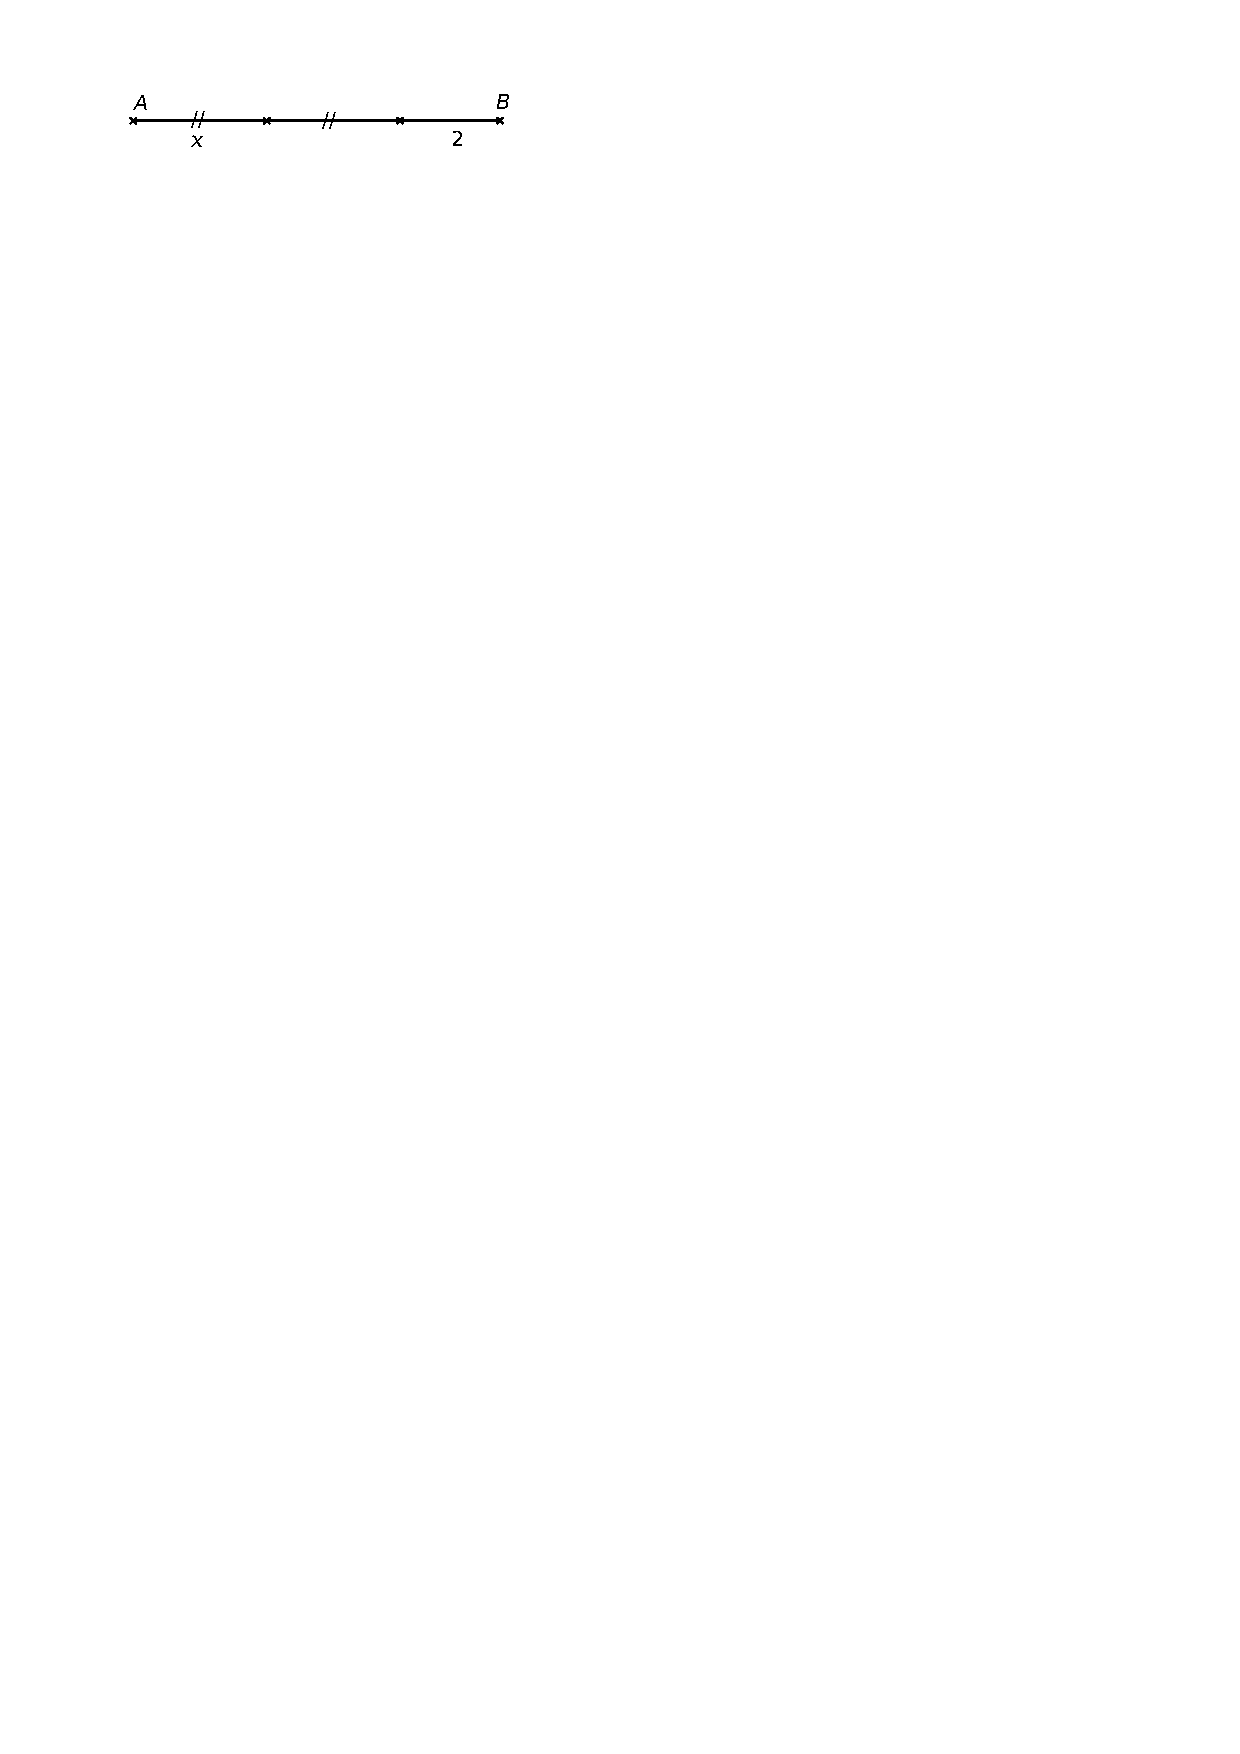
\includegraphics[scale=1.1]{media/fa-10/ligne2.pdf}

AB = \hrulefill

  \task 
  
     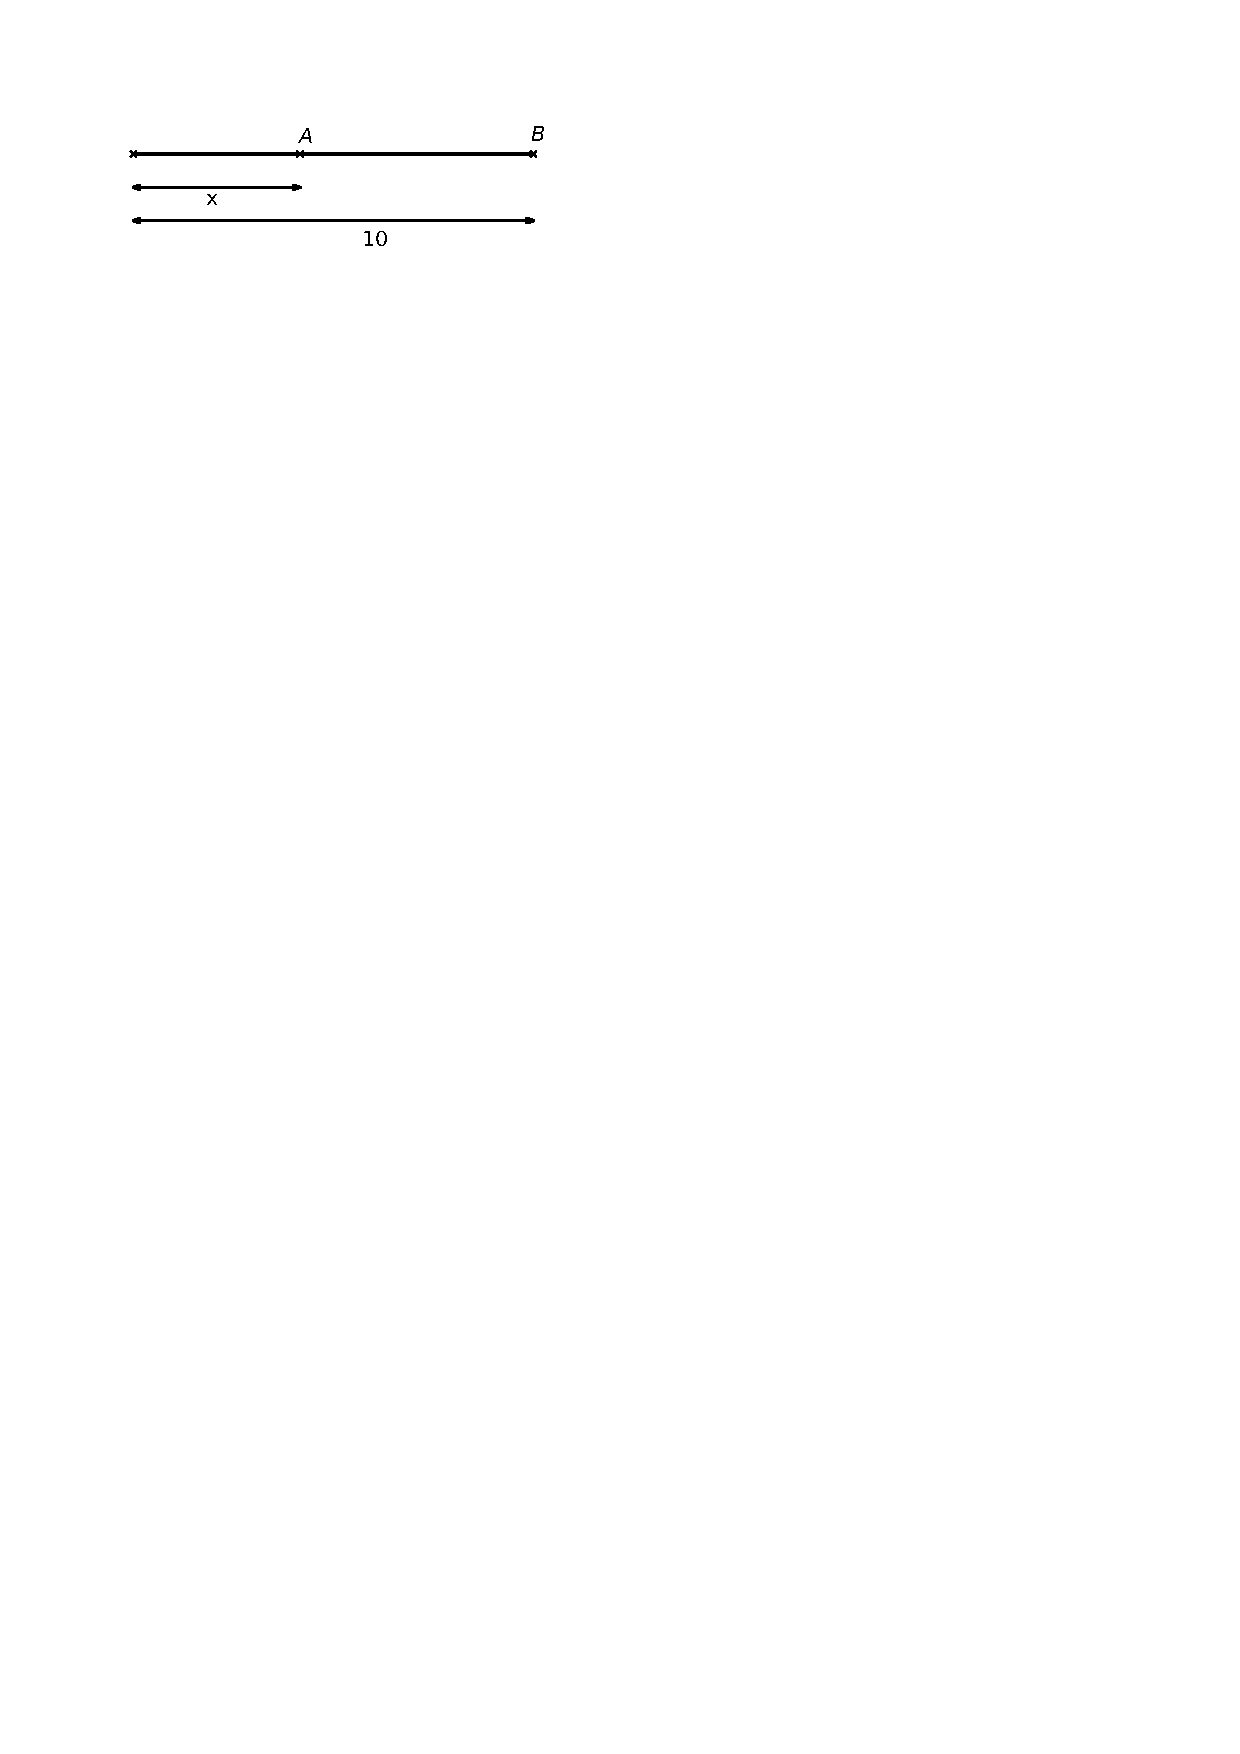
\includegraphics[scale=1.1]{media/fa-10/ligne3.pdf}

AB = \hrulefill

\end{tasks}
}
{3}
\end{exop}

\begin{exol}{FA62}{88}{2}
\end{exol}

\begin{exol}{FA76}{90}{2}
\end{exol}

\begin{exol}{FA77}{90}{2}
\end{exol}

%\begin{resolu}{Problème}
%	{Jean, Marc et Julie se rendent dans un magasin de bonbons. Marc achète deux fois plus de bonbons que Jean. Julie achète 5 bonbons de moins que Jean. Le total des achats est de \tunit{15}{\fr}
%
%\begin{tasks}(1)
%
%    \task Quelle est l'inconnue~?
%    \task Exprime algébriquement, en fonction de x, combien chaque enfant a reçu de bonbons.
%    \task Pose l'équation. 
%    \task Est-ce que 5 est la solution de cette équation~?
%\end{tasks}
%
%Solutions~:
%
% \begin{tasks}(1)   
%    \task Le nombre de bonbons achetés par Jean
%
%    \task x = Bonbons de Jean
%
%        2x = Bonbons de Marc
%
%        x-5= Bonbons de Julie
%
%    \task $x+2x+x-5=15$
%
%        $<-> 4x-5=15 $
%    \task Oui car $4\cdot5-5=15$
%\end{tasks}
%
%}
%{3}    
%\end{resolu}
%    
%\begin{exo}
%{La mère de  Justine à 4 ans de plus que le double de l'âge de Justine. La somme des âges de Justine et sa mère vaut 40 ans. 
%
%\begin{tasks}
%   \task Quelle est l'inconnue~?
%   \task Exprime l'âge de la maman en fonction de celui de Justine.
%   \task Pose l'équation.
%   \task Est-ce que 12 est la solution de l'équation~?
%\end{tasks}
%
%}
%{3}
%\end{exo}
%
%\begin{exo}
%{La somme d'un nombre, de son double et de son quart vaut 28.
%
%\begin{tasks}
%   \task Quelle est l'inconnue~?
%   \task Pose l'équation.
%   \task Est-ce que 10 est la solution de l'équation~?
%   \task Trouve la solution.
%\end{tasks}
%}
%{3}
%\end{exo}
%
%
%\begin{exo}
%{La différence d'un nombre et de son tiers vaut 6.
%
%\begin{tasks}
%   \task Quelle est l'inconnue~?
%   \task Pose l'équation.
%   \task Est-ce que 12 est la solution de l'équation~?
%   \task Trouve la solution.
%\end{tasks}
%}
%{3}
%\end{exo}
%\newpage
%\begin{exo}
%{ Voici l'angle $\widehat{AOB}$. Il mesure x et est coupé par la demi-droite d, la bissectrice de cet angle. Nathan aimerait exprimer algébriquement la mesure de l'angle $\widehat{dOB}$. Aide Nathan.
%
%\begin{center}
%
%         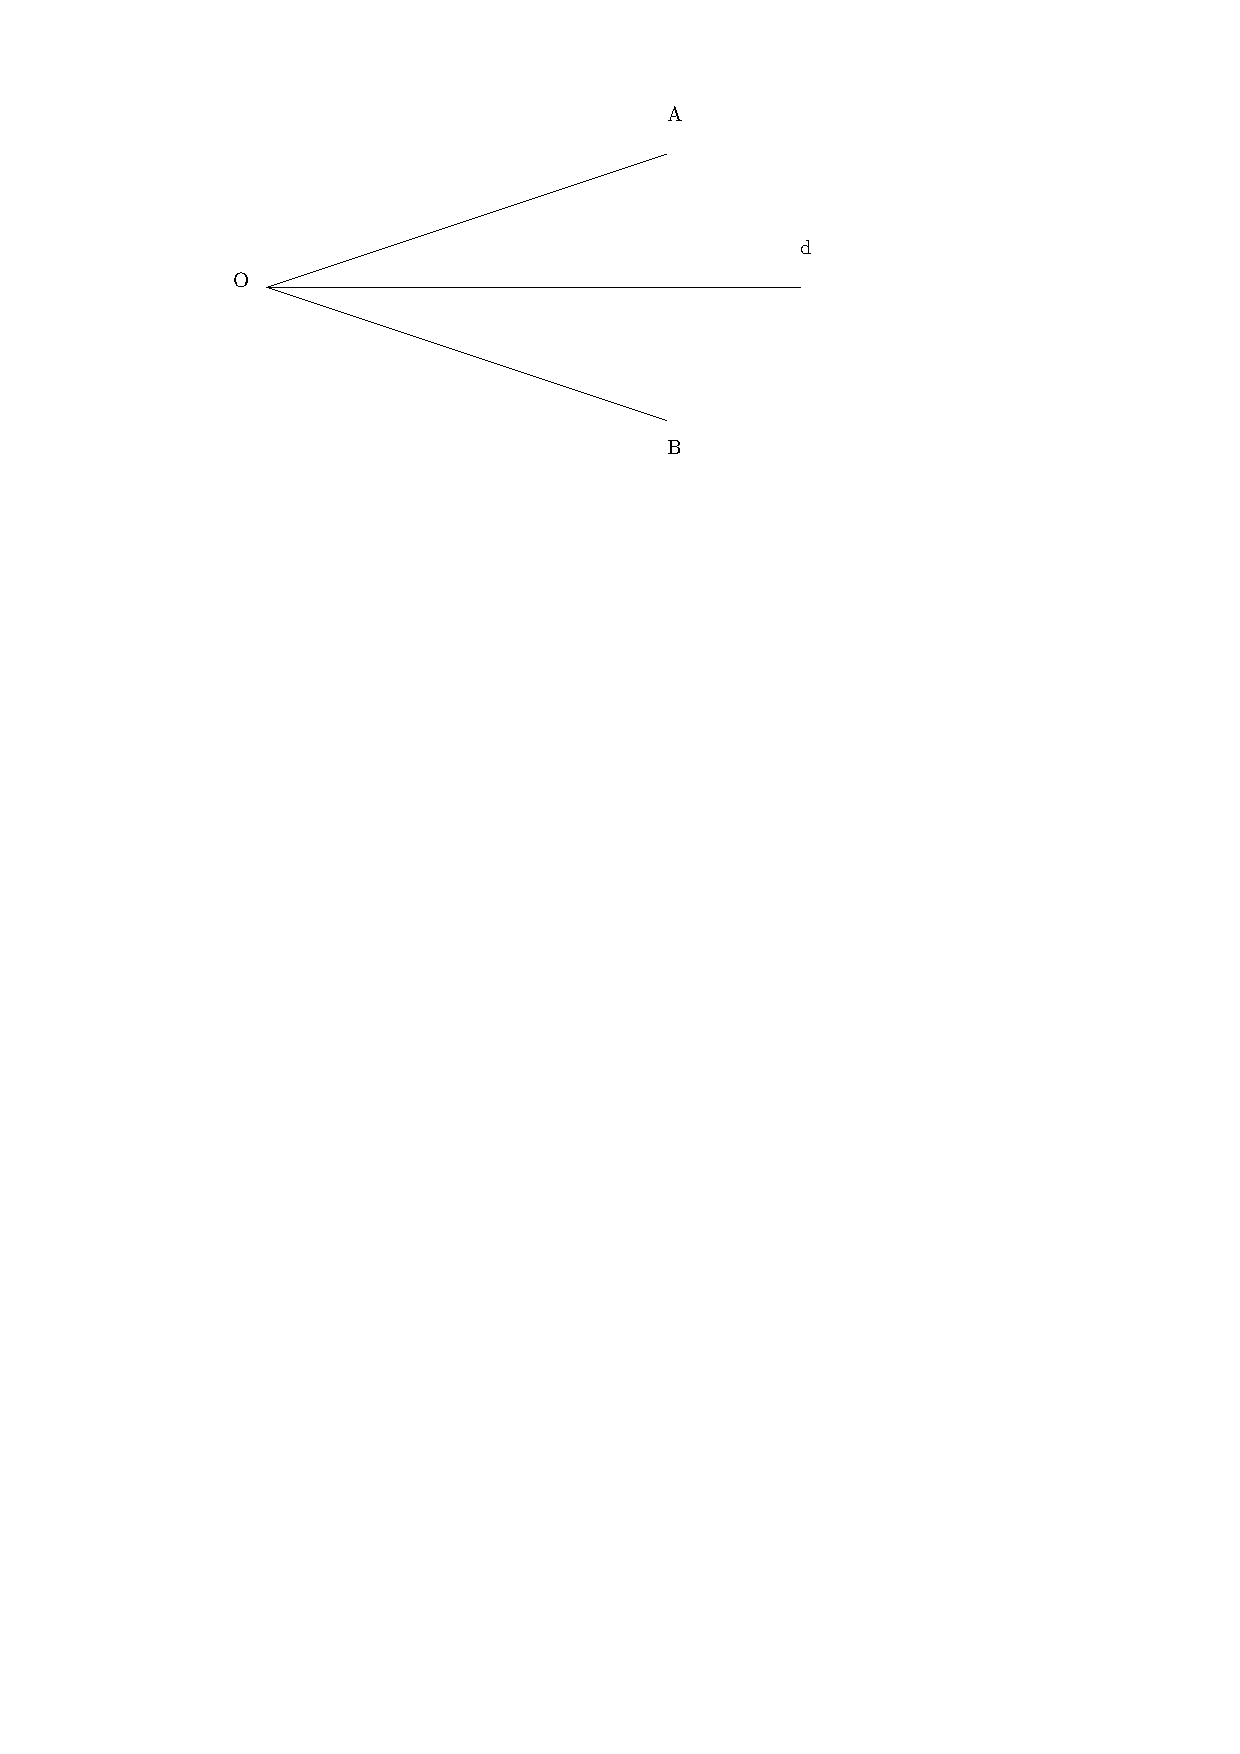
\includegraphics[scale=1.0]{media/fa-10/bissectrice.pdf}
%\end{center}
%}
%{3}
%\end{exo}
%
%\begin{exol}{FA81}{91}{2}
%\end{exol}
%
%
%
%
%
%\begin{FLP}{99}{2}
%\end{FLP}
%
\end{document}
